\documentclass[12,french]{report} 
\usepackage{geometry}
\geometry{vmargin=3cm, hmargin=3cm}
\usepackage[T1]{fontenc}
\usepackage[utf8]{inputenc}
\usepackage[french]{babel}
\usepackage{graphicx}
\usepackage{amsmath}
\usepackage{amssymb}
\usepackage{sectsty}
\usepackage{authblk}
\usepackage{algpseudocode}
\usepackage{algorithm}
\usepackage{xspace}
\usepackage{mathtools}
\usepackage{mathrsfs}
\usepackage{enumitem}
\usepackage{titlesec}
\usepackage{hyperref}
\usepackage{xcolor}
\usepackage[justification=centering]{caption}
\usepackage{float}
\usepackage{tabto}

\usepackage{listings}
\usepackage{cleveref}

\renewcommand{\lstlistingname}{Code}
%\renewcommand{\figurename}{Fig.}

\lstdefinestyle{chstyle}{%
backgroundcolor=\color{gray!12},
basicstyle=\ttfamily\small,
showstringspaces=false,
numbers=left}

%\AddThinSpaceBeforeFootnotes
%\FrenchFootnotes

\titleformat{\chapter}[hang]{\bf\Huge}{\thechapter.}{2pc}{}
\titlespacing*{\chapter}{10pt}{0pt}{40pt}[0pt]
\newcommand{\HRule}{\rule{\linewidth}{0.5mm}}

\providecommand{\keywords}[1]{\textbf{\textit{Keywords:}} #1}
\bibliographystyle{apalike}

\usepackage{hyperref}

\begin{document}
\hypersetup{pdfborder=0 0 0}

\begin{titlepage}

\begin{center}
	\vspace*{\stretch{1}}
	\textsc{\LARGE Institut national des sciences appliquées de Rouen} 
	\vspace{5mm}\\
	
\includegraphics[width=0.4\textwidth]{./Images/insa}\\[1.0 cm]

	\textsc{\Large Projet MMSN GM3 - Vague 3 - Sujet 4}\\[0.6cm]

	% Title
	\HRule \\[0.5cm]
	{ \Huge \bfseries Etude des erreurs sur la méthode du Gradient Conjugué}\\[0.2cm]
	\HRule \\[0.75cm]

	
\includegraphics[width=0.6\textwidth]{./Images/Page_de_garde}\\[0.9 cm]

	% Author and supervisor
	\begin{minipage}{0.4\textwidth}
		\begin{flushleft} \large
			\emph{Auteurs:}\\
			Thibaut \textsc{André-Gallis} \\
			{\small\href{mailto:thibaut.andregallis@insa-rouen.fr}{thibaut.andregallis@insa-rouen.fr}} \\
			Kévin \textsc{Gatel} \\
			{\small\href{mailto:kevin.gatel@insa-rouen.fr}{kevin.gatel@insa-				rouen.fr}}
		\end{flushleft}
	\end{minipage}
	\begin{minipage}{0.4\textwidth}
		\begin{flushright} \large
			\emph{Enseignants:} \\
			Mathieu \textsc{Bourgais} \\
			{\small\href{mailto:mathieu.bourgais@insa-rouen.fr}								{mathieu.bourgais@insa-rouen.fr}}\\
		\end{flushright}
	\end{minipage}
	\vspace*{\stretch{1}}

	\vfill
	{\large 6 Juin 2021}
\end{center}
\end{titlepage}

\tableofcontents

%\listoffigures

\renewcommand{\chaptername}{}
\chapter*{Introduction} %thib
\addcontentsline{toc}{chapter}{Introduction}

\chapter{Présentation du problème} %kev

L'objectif est donc d'étudier les erreurs que fait la machine en utilisant l'arithmétique flottante plutôt que l'ensemble théorique des réels.\\

 Ces erreurs seront étudiées sur la solution du problème linéaire $Ax=b$ avec la méthode du gradient conjugué. En choisissant la matrice $A$ de dimension 4 définie comme ci-dessous :\\

\begin{figure}[H]
	\center
	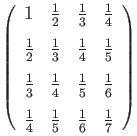
\includegraphics[width=0.2\textwidth]{./Images/H_4}
	\caption{Matrice de Hilbert de dimension 4}
\end{figure}

Le nombre d'étape pour trouver la solution sera en théorie inférieur ou égale à 4 (assuré par la méthode du gradient conjugué).\\

En notant $K_2(A)$ le conditionnement 2 de A tel que :\footnote{conditionnement obtenu sur Matlab}
$$K_2(a)= 1.5514*10^4$$

On a l'inégalité du conditionnement pour majorer l'erreur :
$$\frac{||\Delta x||_{2}}{||x||_2}\leq K_2(A)\frac{||\Delta b||_{2}}{||b||_2}$$

Le test d'arrêt est de la forme $$tol^2*(b,b) > (r,r) $$
avec $(\bullet,\bullet)$ le produit scalaire usuel et $tol=10^{-10}$.\\

Enfin, le vecteur $b$ est choisi comme ci-dessous :

$$b_i=\sum_{k=1}^4a_{ik}$$

de manière à avoir 
$$x^T=\left(\begin{array}{cccc}
1 & 1 & 1 & 1\end{array}\right)$$




\chapter{Vecteur résidu $r$} %thib

\section{Etape 0}

\section{Etape 1}

\section{Etape 2}

\section{Etape 3}

\section{Etape 4}

\chapter{Vecteur solution $x$} %kev

\section{Etape 1}

\section{Etape 2}

\section{Etape 3}

\section{Etape 4}

\chapter{Analyse numérique du problème} %kev

Analysons maintenant le problème numériquement. On sait que la solution théorique est
$$x^T=\left(\begin{array}{cccc}
1 & 1 & 1 & 1\end{array}\right)$$

Comparons maintenant ce résultat avec celui qu'on a obtenu numériquement au bout de la $4^{eme}$ étape :
$$\hat{x}^T=\left(\begin{array}{cccc}
0.9999999987685677105 & 0.9999999992953791939 & 0.9999999994982825546 & 0.99999999960549057491\end{array}\right)$$\vspace{0cm}

On peut maintenant obtenir l'erreur absolue pour chaque composante afin d'obtenir le vecteur absolu :\footnote{calcul effectué sur \textit{wolframalpha.com}}

$$\varepsilon_{abs}=\left(\begin{array}{cccc}
1.2314322895*10^{-9} & 7.046208061*10^{-10} & 5.017174454*10^{-10} & 3.9450942509*10^{-10} \end{array}\right)$$\vspace{0cm}

On remarque que l'on obtient le même vecteur pour le vecteur erreur relative puisqu'on divise toutes les composantes par 1 :

$$\varepsilon_{rel}=\left(\begin{array}{cccc}
1.2314322895*10^{-9} & 7.046208061*10^{-10} & 5.017174454*10^{-10} & 3.9450942509*10^{-10} \end{array}\right)$$

On observe des erreurs beaucoup plus élevées que celles obtenues localement. En effet pour une étude local on obtenait des erreurs d'ordre de grandeur d'environ $10^{-17}$ alors qu'ici il est d'environ $10^{-10}$. Une différence de $10^{7}$ qui n'est pas négligeable.\\

Cependant, on peut souligner l'efficacité de la méthode car en seulement 4 itérations l'erreur de la solution obtenue par rapport à celle théorique est de seulement $10^{-9}$. Si l'on veut obtenir plus de précision il suffit de diminuer la tolérance et d'observer davantage d'étapes.





\chapter*{Conclusion} %thib
\addcontentsline{toc}{chapter}{Conclusion}

\chapter*{Annexe}

\end{document}
